% COMPOSITE

\subsection{Part A - Experimental Errors and Uncertainty}

\subsubsection{Pre--Lab Questions}

\begin{enumerate}
	\item Explain the difference between accuracy and precision.

	      \textbf{Accuracy is how close a measured or average value is to the true value, whereas precision is how close the individual measured values are to one another (repeatability)}

	\item Name a statistical quantity that can be used to indicate an accuracy level.

	      \textbf{Percent Error can be used to indicate an accuracy level.}

	\item Name a statistical quantity that can be used to indicate a precision level.

	      \textbf{Standard Deviation can be used to indicate a precision level.}

	\item To what level of accuracy (\SI{1}{cm}, \SI{0.1}{cm}, \SI{0.01}{cm}, \SI{0.001}{cm}) can the ruler used to measure the lengths of the pencil in Table 1 of the Lab 1 Instructions Sheet be read?

	      \textbf{It can be read to \SI{0.01}{cm}, because the measurements are accurate to this degree.}
\end{enumerate}

\newpage

\begin{center}
	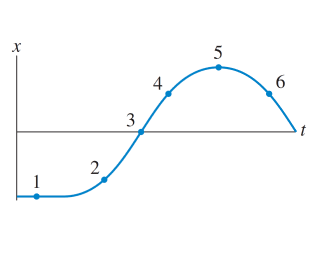
\includegraphics[width=0.8\textwidth]{/Users/max/course-manager/data/semester/Spring 2025/course/PHY2111/chapter/Kinematics in One Dimension/section/Lab 1/figures/figure_1.png
	}
\end{center}

In the above cartoon, three bullseyes have been drawn representing dart boards. Each has had six darts thrown at it by three different throwers, $A$, $B$, and $C$, respectively.

\begin{enumerate}
	\setcounter{enumi}{4}
	\item Which thrower is the most accurate? Explain your choice.

	      \textbf{Thrower $B$ is the most accurate because, on average, their darts cluster closest to the center.}

	\item Which thrower is the most precise? Explain your choice.

	      \textbf{Thrower $C$ is the most precise because the grouping is closest together, regardless of the distance from the center.}

	\item Which would you want on your team? Explain your choice.

	      \textbf{Ideally, a thrower who is both accurate and precise, but I would choose thrower $B$ because they have a possibility of actually hitting the center, rather than thrower $C$, who would almost certainly never hit the center.}

\end{enumerate}

\subsubsection{Post--Lab Questions}

\paragraph{Part 1}~

A student measures the value of the acceleration due to gravity several times and obtains the following results (all in $\SI{}{m/s^2}$ units):
\begin{center}
	9.95, 10.10, 9.97, 9.99, and 10.02
\end{center}

Given: The accepted value for the acceleration due to gravity on Earth is $\SI{9.81}{\frac{m}{s^2}}$.

\newpage

\begin{remark}
	~
	\begin{enumerate}
		\item Mean
		      \begin{align*}
			      \overline{x} &= \frac{9.95+10.10+9.97+9.99+10.02}{5} = \SI{10.006}{\frac{m}{s^2}}
		      \end{align*}
		\item Standard Deviation
		      \begin{align*}
			      \left( 9.95-10.006 \right)^2 &= 0.003136 \\
			      \left( 10.10-10.006 \right)^2 &= 0.008836 \\
			      \left( 9.97-10.006 \right)^2 &= 0.001296 \\
			      \left( 9.99-10.006 \right)^2 &= 0.000256 \\
			      \left( 10.02-10.006 \right)^2 &= 0.000196
			      .\end{align*}
		      Sum: $0.01372$
		      \begin{align*}
			      \sigma &= \sqrt{\frac{0.01372}{5-1}} = 0.0585662
			      .\end{align*}
	\end{enumerate}
\end{remark}

\begin{enumerate}
	\setcounter{enumi}{7}
	\item Determine the uncertainty range for this set of data, using any calculation tool at your disposal.  Please record the uncertainty range here with appropriate significant figures and units as discussed in the above pages.
	      \[
		      g = 10.01 \pm \SI{0.06}{\frac{m}{s^2}}
		      .\]
	\item Determine both the accuracy and precision levels in percentage form.  Show your work here.
	      \begin{align*}
		      \text{Percent Error} &= \frac{\abs{ 10.01 - 9.81 }}{9.81} \times \SI{100}{\percent} \approx \SI{2.0}{\percent} \\
		      \text{Precision Level} &= \frac{0.06}{10.01} \times \SI{100}{\percent} \approx \SI{0.6}{\percent}
		      .\end{align*}
	\item Do random errors alone seem to account for any inaccuracies from the accepted value, or does a systematic error appear to be present?  Explain your reasoning.
	      \begin{align*}
		      \SI{10.01}{\frac{m}{s^2}} - \SI{9.81}{\frac{m}{s^2}} &= \SI{0.2}{\frac{m}{s^2}} \\
		      \frac{\SI{0.2}{\frac{m}{s^2}}}{\sigma \, \text{or} \, 0.06} &= 3.33
		      .\end{align*}
	      \textbf{Since the measured mean differs from the expected value ($\SI{9.81}{\frac{m}{s^2}}$) by about 3 times the standard deviation, random errors alone do not seem to account for the total inaccuracy of the measurements.}
\end{enumerate}

\newpage

\paragraph{Part 2}~

We may not always be able to determine an accuracy level using a percent error calculation when an accepted value for a quantity is unknown. However, if we have multiple ways of determining a quantity, such as independent measuring methods or theories, we can compare two different results for the same quantity using a percent difference. Comparing the uncertainty range between the two methods is very useful as well.

Later on in Module 2, we will study frictional forces along with coefficients of friction which are unitless numbers that describe the amount of friction between various surfaces. Let us compare a set of measurements for a friction coefficient between a wooden and rubber surface using two different methods of measurement: a simple pulling technique versus an incline sliding technique. Here's the data:

\begin{enumerate}
	\setcounter{enumi}{10}
	\item Complete the values in the table for the uncertainty ranges and precision levels for each set and find the percent difference between the two sets.  Show your worked out calculations below.
\end{enumerate}

\begin{table}[htpb]
	\centering
	\caption{Coefficients of Friction between wood and rubber surfaces}
	\label{tab:Table2.1}
	\begin{tblr}{|c|c|}
		\hline
		Direct Pulling Method & Incline Plane Method \\
		\hline
		0.72                  & 0.71                 \\
		\hline
		0.70                  & 0.91                 \\
		\hline
		0.79                  & 0.66                 \\
		\hline
		0.74                  & 0.79                 \\
		\hline
		0.75                  & 0.87                 \\
		\hline
	\end{tblr}
\end{table}

\begin{remark}
	\begin{enumerate}
		~
		\item Direct Pulling Method
		      \begin{align*}
			      \overline{x}_{\mathrm{pull}} &= \frac{0.72 + 0.70 + 0.79 + 0.74 + 0.75}{5} = 0.74 \\
			      \sigma_{\mathrm{pull}} &\approx 0.034 \longleftarrow \text{Calculated using Google Sheets}
			      .\end{align*}
		      Uncertainty Range $= 0.74 \pm 0.03$

		      Precision Level $= \frac{0.034}{0.74} \times \SI{100}{\percent} \approx \SI{4.6}{\percent}$
		\item Incline Plane Method
		      \begin{align*}
			      \overline{x}_{\mathrm{incline}} &= \frac{0.71 + 0.91 + 0.66 + 0.79 + 0.87}{5} = 0.788 \\
			      \sigma_{\mathrm{incline}} &\approx 0.11 \longleftarrow \text{Calculated using Google Sheets}
			      .\end{align*}
		      Uncertainty Range $= 0.79 \pm 0.11$

		      Precision Level $= \frac{0.11}{0.79} \times \SI{100}{\percent} \approx \SI{14}{\percent}$
	\end{enumerate}
\end{remark}

\textbf{The percent difference between the two average values is}
\[
	\frac{\abs{ 0.79-0.74 }}{\left( 0.74+0.79 \right) \divisionsymbol 2} \times \SI{100}{\percent}
	= \SI{6.5}{\percent}
	.\]

\begin{table}[htpb]
	\centering
	\caption{Coefficients of Friction between wood and rubber surfaces}
	\label{tab:Table2.2}
	\begin{tblr}{
			hlines = {2-4}{solid},
			hline{7-10} = {solid},
			vline{2-4} = {solid},
			vline{1} = {7-10}{solid},
		}
		                     & Direct Pulling Method               & Incline Plane Method \\
		                     & 0.72                                & 0.71                 \\
		                     & 0.70                                & 0.91                 \\
		                     & 0.79                                & 0.66                 \\
		                     & 0.74                                & 0.79                 \\
		                     & 0.75                                & 0.87                 \\
		Uncertainty Range    & $0.74 \pm 0.03$                     & $0.79 \pm 0.11$      \\
		Precision Level (\%) & \SI{4.6}{\percent}                  & \SI{14}{\percent}    \\
		Percent Difference   & \SetCell[c=2]{c} \SI{6.5}{\percent}                        \\
	\end{tblr}
\end{table}

\begin{enumerate}
	\setcounter{enumi}{11}
	\item Which data set seems to be more reliable and why?  Does this set have less random or systematic error?

	      \textbf{The Direct Pulling Method has a significantly smaller standard deviation, so it is more precise and probably more reliable in terms of random error. There isn't really a value to compare against, so there doesn't seem to be a large systematic offset.}

	\item Given the percent difference between the two sets, do you think the two sets provide a statistically different value for those coefficients, or do you think they are statistically the same? Use the uncertainty ranges to help explain this.

	      \textbf{The difference between the means ($0.788-0.74 \approx 0.05$) is small, and the uncertainty ranges overlap. This means that the sets are not statistically much different.}

	\item Comparing the two uncertainty ranges, does any of the data appear to be suffering from any systematic effects?  Why or why not?

	      \textbf{There is no strong indication of a systematic effect in one method vs. the other. In other words, no single shift is making all values bigger or smaller in a way that is outside the other method's range.}
\end{enumerate}
